\section{Combinar}
\par{Este filtro consiste en realizar una combinación de dos imágenes que dependa de un número real $\alpha$ entre 0 y 255.}
\par{Cabe destacar que este filtro permite reutilizar cálculos debido a dos factores. Uno de ellos es la forma que tiene cada píxel generado en la imagen resultante, que consiste en que si se tienen una imagen $A$ y una imagen $B$ de tamaño $m \times n$ entonces el píxel de la imagen generada ${I_{AB}}^{i, j}$ se calcula de la siguiente forma:}
\[ {I_{AB}}^{i,j} = \dfrac{\alpha * ( {I_{A}}^{i,j} - {I_{B}}^{i,j} )}{255.0} + {I_{B}}^{i,j} \]
\par{El otro factor es que nuestro filtro está optimizado para casos en los que la imagen $B$ es el reflejo vertical de la imagen $A$. Es decir que se da que ${I_{A}}^{i,j} = {I_{B}}^{i,n - j + 1}$ como se puede apreciar en la siguiente figura.}

\begin{figure}[h!]
\centering
\begin{minipage}{.5\textwidth}
\centering
\captionsetup{justification=centering}
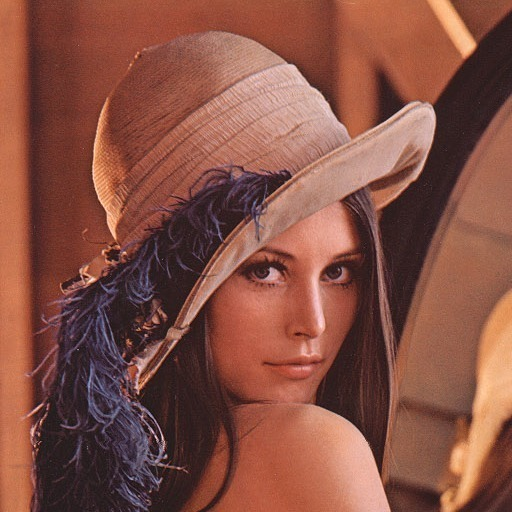
\includegraphics[width=5cm, height=5cm]{imagenes/CombinarOriginal.jpg}
\label{}
\end{minipage}\hfill
\begin{minipage}{.5\textwidth}
\centering
\captionsetup{justification=centering}
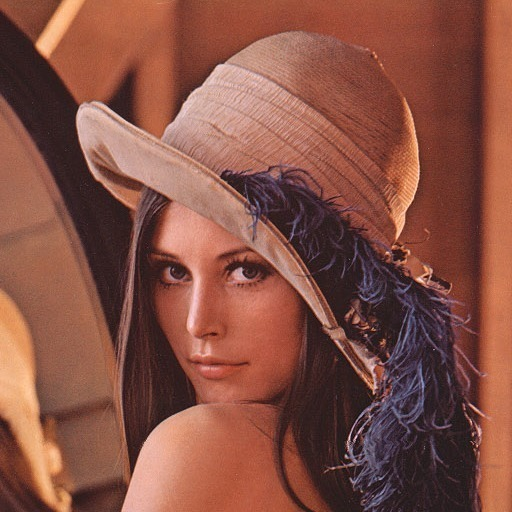
\includegraphics[width=5cm, height=5cm]{imagenes/CombinarReflejo.jpg}
\label{}
\end{minipage}
\caption[center]{Se muestra la imagen $A$ del lado izquierdo con la imagen $B$, el reflejo vertical de A, en la parte derecha.}
\end{figure}

\par{Entonces se tiene que}
\begin{align}
{I_{AB}}^{i,j} &= \dfrac{\alpha * ( {I_{A}}^{i,j} - {I_{B}}^{i,j} )}{255.0} + {I_{B}}^{i,j} \textup{     por la fórmula del filtro} \nonumber \\
&= \dfrac{\alpha * ( {I_{A}}^{i,j} - {I_{A}}^{i,n - j + 1} )}{255.0} + {I_{A}}^{i,n - j + 1} \textup{    dado que } {I_{A}}^{i,j} = {I_{B}}^{i,n - j + 1}
\end{align}

y análogamente

\begin{align}
{I_{AB}}^{i,n - j + 1} &= \dfrac{\alpha * ( {I_{A}}^{i,n - j + 1} - {I_{B}}^{i,n - j +1} )}{255.0} + {I_{B}}^{i,n - j + 1}  \nonumber \\
&= \dfrac{\alpha * ( {I_{A}}^{i,n - j + 1} - {I_{A}}^{i,j} )}{255.0} + {I_{A}}^{i,j}
\end{align}

\par{Así, se obtiene}

\begin{align}
{I_{AB}}^{i,n - j + 1} &= -1 * \dfrac{\alpha * [-1 * ( {I_{A}}^{i,n - j + 1} - {I_{A}}^{i,j} )]}{255.0} - {I_{A}}^{i,n - j + 1} + {I_{A}}^{i,n - j + 1} + {I_{A}}^{i,j} \nonumber \\
&= -1 * \Big[ \dfrac{\alpha * ( {I_{A}}^{i,j} - {I_{A}}^{i,n - j + 1} )}{255.0} + {I_{A}}^{i,n - j + 1} \Big] + {I_{A}}^{i,n - j + 1} + {I_{A}}^{i,j} \nonumber \\
&= -1 * ( {I_{AB}}^{i,j} - {I_{A}}^{i,n - j + 1} ) + {I_{A}}^{i,j} \textup{usando la igualdad de (2)}
\end{align}

\par{Estos cálculos muestran que luego de hacer el procesamiento para generar un píxel de la parte izquierda de la imagen resultante se puede obtener el píxel que corresponde a la mitad derecha con pocos cálculos más. Más aún, si se denomina}
\[ P = \dfrac{\alpha * ( {I_{A}}^{i,j} - {I_{A}}^{i,n - j + 1} )}{255.0} \]
se consigue
\[ {I_{AB}}^{i,j} = P + {I_{A}}^{i,n - j + 1} \]
y
\[ {I_{AB}}^{i,n - j + 1} = -P + {I_{A}}^{i,j} \]
dando lugar a menos cálculos necesarios.

\subsection{Código C}
\par{A continuación se presenta el pseudocódigo detallado del filtro.}
\par{Clamp es una función que controla la saturación.}
\begin{algorithm}[h!]
\caption{Clamp}
\begin{algorithmic}
  \Function{clamp}{$pixel: ~float$}  $\to \texttt{float}$
	\If{$pixel < 0.0$}
		\State \Return $0.0$
	\Else
		\If{$pixel > 255.0$}
			\State \Return $255.0$
		\Else
			\State \Return $pixel$
		\EndIf
	\EndIf
\EndFunction
\end{algorithmic} 
\end{algorithm}

\par{Combine realiza los cálculos correspondientes determinados por el filtro.}
\begin{algorithm}[h!]
\caption{Combine}
\begin{algorithmic}
  \Function{combine}{$a: ~unsigned~ char, ~b: ~unsigned~ char, ~\alpha: ~float$}  $\to \texttt{float}$
	\State float $af \gets a$
	\State float $bf \gets b$
	\State \Return $\dfrac{\alpha * (af - bf)}{255.0} + bf$
\EndFunction
\end{algorithmic} 
\end{algorithm}

\par{Combinar llama a las dos funciones ya explicadas y obtiene 2 píxeles con los que operar para luego dejar el resultado en la imagen destino.}
\begin{algorithm}[h!]
\caption{Combinar}
\begin{algorithmic}
  \Function{combinar}{src: *unsigned char, dst: *unsigned char, cols: int, filas: int, srcRowSize: int, dstRowSize: int, $\alpha$: float}
	\State $unsigned~ char~ (*srcMatrix)[srcRowSize] = (unsigned~ char (*)[srcRowSize])~ src$
	\State $unsigned~ char~ (*dstMatrix)[dstRowSize] = (unsigned~ char (*)[dstRowSize])~ dst$
	\For{$f \gets 0~..~filas-1$}
		\For{$c \gets 0~..~cols-1$}
			\State $bgra_t* p_{sa} \gets (bgra_t*)$ \& $srcMatrix[f][c * 4]$
			\State $bgra_t* p_{sb} \gets (bgra_t*)$ \&$srcMatrix[f][(cols - c -1) * 4]$
			\State $bgra_t *p_d \gets (bgra_t*)$ \&$dstMatrix[f][c * 4]$
			\State $p_d$->$b \gets$ \Call{clamp}{\Call{combine}{$p_{sa}$->$b$, $p_{sb}$->$b, \alpha$}}
			\State $p_d$->$g \gets$ \Call{clamp}{\Call{combine}{$p_{sa}$->$g, p_{sb}$->$g, \alpha$}}
			\State $p_d$->$r \gets$ \Call{clamp}{\Call{combine}{$p_{sa}$->$r, p_{sb}$->$r, \alpha$}}
			\State $p_d$->$a \gets$ \Call{clamp}{\Call{combine}{$p_{sa}$->$a, p_{sb}$->$a, \alpha$}}
		\EndFor
	\EndFor
\EndFunction
\end{algorithmic} 
\end{algorithm}
	
\subsection{Código ASM}
\par{Dado que cada píxel tiene 4 bytes y los registros XMM tienen 16 bytes, se levantan 4 píxeles contiguos desde la posición $i,j$ y otros 4 píxeles desde la $i, n-j+1$ en otro registro.}
\par{Se mostrará cómo se genera el píxel $I_{i,j}$ de la imagen resultante.}
%\xmmb{$P_{j+3}A$}{$P_{j+3}R$}{$P_{j+3}G$}{$P_{j+3}B$}{$P_{j+2}A$}{$P_{j+2}R$}{$P_{j+2}G$}{$P_{j+2}B$}{$P_{j+1}A$}{$P_{j+1}R$}{$P_{j+1}G$}{$P_{j+1}B$}{$P_jA$}{$P_jR$}{$P_jG$}{$P_jB$}
\par{Se levantan 4 píxeles de la mitad izquierda en el registro XMM1:}
\par{\textbf{XMM1:}}
\xmmb{$A_{j+3}$}{$R_{j+3}$}{$G_{j+3}$}{$B_{j+3}$}{$A_{j+2}$}{$R_{j+2}$}{$G_{j+2}$}{$B_{j+2}$}{$A_{j+1}$}{$R_{j+1}$}{$G_{j+1}$}{$B_{j+1}$}{$A_j$}{$R_j$}{$G_j$}{$B_j$}
\par{y 4 en espejo de la mitad derecha en XMM3:}\\
\par{\textbf{XMM3:}}
\xmmb{$A_{n-j+4}$}{$R_{n-j+4}$}{$G_{n-j+4}$}{$B_{n-j+4}$}{$A_{n-j+3}$}{$R_{n-j+3}$}{$G_{n-j+3}$}{$B_{n-j+3}$}{$A_{n-j+2}$}{$R_{n-j+2}$}{$G_{n-j+2}$}{$B_{n-j+2}$}{$A_{n-j+1}$}{$R_{n-j+1}$}{$G_{n-j+1}$}{$B_{n-j+1}$}

Teniendo
\par{\textbf{XMM9:}}
\xmmb{$0$}{$0$}{$0$}{$0$}{$0$}{$0$}{$0$}{$0$}{$0$}{$0$}{$0$}{$0$}{$0$}{$0$}{$0$}{$0$}
se ejecuta la instrucción \textbf{punpcklbw xmm1, xmm9} que da como resultado
\par{\textbf{XMM1:}}
\xmmb{$0$}{$A_{j+1}$}{$0$}{$R_{j+1}$}{$0$}{$G_{j+1}$}{$0$}{$B_{j+1}$}{$0$}{$A_j$}{$0$}{$R_j$}{$0$}{$G_j$}{$0$}{$B_j$}
\par{y luego \textbf{punpcklwd xmm1, xmm9} para seguir desempaquetando. De esta forma quedan 4 bytes para cada componente del píxel y se podrán convertir a floats para mayor precisión en los cálculos que implican el $\alpha$.}
\par{\textbf{XMM1:}}
\xmmb{$0$}{$0$}{$0$}{$A_j$}{$0$}{$0$}{$0$}{$R_j$}{$0$}{$0$}{$0$}{$G_j$}{$0$}{$0$}{$0$}{$B_j$}
\par{Se copió el contenido de XMM1 a XMM10 y con el registro que contenía al píxel $n-j+4$, obtenido de forma análoga a como se obtuvo el píxel $j$}
\par{\textbf{XMM8:}}
\xmmb{$0$}{$0$}{$0$}{$A_{n-j+4}$}{$0$}{$0$}{$0$}{$R_{n-j+4}$}{$0$}{$0$}{$0$}{$G_{n-j+4}$}{$0$}{$0$}{$0$}{$B_{n-j+4}$}
\par{se realizaron las restas entre componentes (\textbf{psubd xmm10, xmm8}) antes de convertir a float el registro XMM10 (\textbf{cvtdq2ps xmm10, xmm10}) dado que realizar la resta con float es una operación mucho más costosa que con enteros y además no había chances de perder precisión con la resta.}
\par{\textbf{XMM10:}}
\xmmdw{$A_j - A_{n-j+4}$}{$R_j - R_{n-j+4}$}{$G_j - G_{n-j+4}$}{$B_j - B_{n-j+4}$}
\par{Se multiplicó por $\alpha$ al registro XMM10 (\textbf{mulps xmm10, xmm0}) y luego se dividió por $255.0$ (\textbf{divps xmm10, xmm14}) obteniéndose}
\par{\textbf{XMM10:}}
\xmmdw{$\dfrac{\alpha * (A_j - A_{n-j+4})}{255.0}$}{$\dfrac{\alpha * (R_j - R_{n-j+4})}{255.0}$}{$\dfrac{\alpha * (G_j - G_{n-j+4})}{255.0}$}{$\dfrac{\alpha * (B_j - B_{n-j+4})}{255.0}$}
\par{Para esto previamente, fuera del ciclo, se había movido el $\alpha$ que había llegado en los últimos 4 bytes de XMM0 a las otras 3 double words del registro con la instrucción \textbf{pshufd xmm0, xmm0, 00000000b} y se había puesto en XMM14 un 255.0 en cada double word declarando \textbf{mascara255: dd 255.0, 255.0, 255.0, 255.0} en \textbf{section .rodata} y luego haciendo \textbf{movdqu xmm14, [mascara255]}. De esta forma, al realizar estas operaciones fuera del ciclo, se minimizan los accesos a memoria y se evita repetir operaciones innecesarias.}
\par{Convirtiendo XMM8 a float con \textbf{cvtdq2ps xmm8, xmm8} y sumándolo a XMM10 con \textbf{addps xmm10, xmm8} se obtuvo}
\par{\textbf{XMM10:}}
\xmmdw{$\dfrac{\alpha * (A_j - A_{n-j+4})}{255.0} + A_{n-j+4}$}{$\dfrac{\alpha * (R_j - R_{n-j+4})}{255.0} + R_{n-j+4}$}{$\dfrac{\alpha * (G_j - G_{n-j+4})}{255.0} + G_{n-j+4}$}{$\dfrac{\alpha * (B_j - B_{n-j+4})}{255.0} + B_{n-j+4}$}
\par{Antes de finalizar el procesamiento, se realizó \textbf{movups xmm15, xmm10} y \textbf{subps xmm15, xmm8} para conservar en XMM15 lo que en el desarrollo de cuentas apareció como P al explicar cómo se podían reutilizar cálculos.}
\par{Por último en el procesamiento de la parte izquierda se convirtió a entero XMM10 con \textbf{cvtps2dq xmm10, xmm10} y se empaquetó con los resultados de los demás píxeles usando instrucciones como \textbf{packusdw xmm11, xmm10} y \textbf{packusdw xmm13, xmm12} para pasar de double word a word,}
\par{\textbf{XMM11:}}
\xmmw{${F_A}_j$}{${F_R}_j$}{${F_G}_j$}{${F_B}_j$}{${F_A}_{j+1}$}{${F_R}_{j+1}$}{${F_G}_{j+1}$}{${F_B}_{j+1}$}
\par{luego \textbf{packuswb xmm13, xmm11} para pasar de word a byte,}
\par{\textbf{XMM11:}}
\xmmb{${F_A}_j$}{${F_R}_j$}{${F_G}_j$}{${F_B}_j$}{${F_A}_{j+1}$}{${F_R}_{j+1}$}{${F_G}_{j+1}$}{${F_B}_{j+1}$}{${F_A}_{j+2}$}{${F_R}_{j+2}$}{${F_G}_{j+2}$}{${F_B}_{j+2}$}{${F_A}_{j+3}$}{${F_R}_{j+3}$}{${F_G}_{j+3}$}{${F_B}_{j+3}$}
\par{y finalmente \textbf{pshufd xmm11, xmm13, 0x1b} quedando todo listo para mover el contenido del registro a donde correspondiera.}
\par{\textbf{XMM11:}}
\xmmb{${F_A}_{j+3}$}{${F_R}_{j+3}$}{${F_G}_{j+3}$}{${F_B}_{j+3}$}{${F_A}_{j+2}$}{${F_R}_{j+2}$}{${F_G}_{j+2}$}{${F_B}_{j+2}$}{${F_A}_{j+1}$}{${F_R}_{j+1}$}{${F_G}_{j+1}$}{${F_B}_{j+1}$}{${F_A}_j$}{${F_R}_j$}{${F_G}_j$}{${F_B}_j$}
\par{Para finalizar la parte derecha se multiplicaron todos los valores de las double words de XMM15 por -1 (\textbf{mulps xmm15, [menos1]} estando menos1 definido en \textbf{rodata} como \textbf{menos1: dd -1.0, -1.0, -1.0, -1.0}) y se prosiguió con las conversiones y sumas como anteriormente.}

	
\subsection{Experimentación}

\subsubsection{Hipótesis}
\par{Nuestra hipótesis era que la implementación en ASM iba a ser mucho más veloz que la de C con el menor nivel de optimización al compilar e incluso que las de C con mayores niveles de optimización.}
\par{Además creíamos que las ejecuciones con la implementación de C iban a presentar un porcentaje de ciclos de clock debidos accesos a memoria mucho mayor que la implementación de ASM.}

\subsubsection{Idea}
\par{Como forma de verificar esto pensamos medir la cantidad de ciclos de clock insumidos en cada caso para la ejecución del filtro. Se realizaron 1000 mediciones y se realizó un gráfico de barras con los promedios obtenidos de dividir cada total de ciclos por la cantidad de iteraciones.}
\par{Por otro lado, se midieron los ciclos de clock relacionados a accesos a memoria con la implementación de ASM y con la de C y se realizaron gráficos de torta para mostrar los porcentajes con respecto al total de ciclos insumidos.}

\subsubsection{Resultados}
\par{En cuanto a las cantidades totales de ciclos de clock se obtuvo el siguiente gráfico.}

\begin{figure}[h!]
\centering
\captionsetup{justification=centering}
	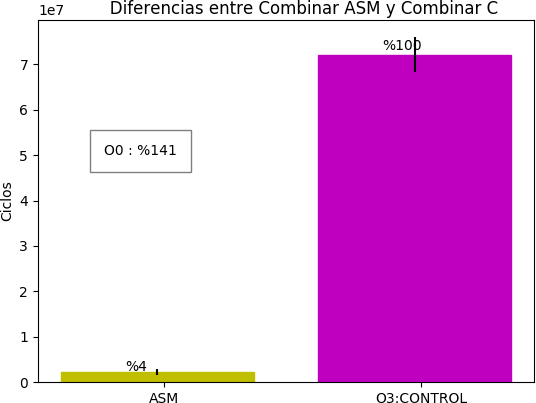
\includegraphics[width = 12 cm, height = 8 cm]{imagenes/CombinarASMvsC.jpeg}
	\caption[center]{Gráfico de barras comparando las implementaciones y diversas optimizaciones.}
\end{figure}

\par{Como se puede apreciar, la implementación de ASM es casi 29 veces más rápida que la menos optimizada de C y también supera ampliamente a las optimizadas, siendo más de 10 veces más rápida. Esto confirma nuestras suposiciones de la mejoría resultante del modelo de procesamiento SIMD.}

\medskip

\par{Con respecto a lo planteado en cuanto a los accesos a memoria, también obtuvimos resultados esperados, visibles en la siguiente figura.}

\begin{figure}[h!]
\centering
\captionsetup{justification=centering}
	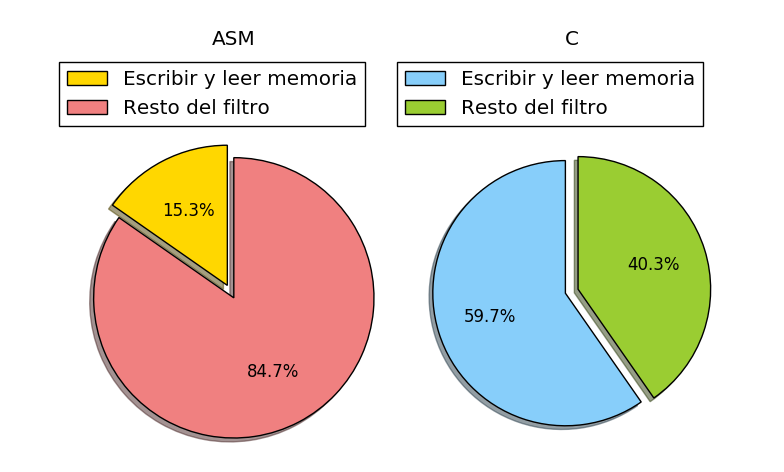
\includegraphics[width = 12 cm, height = 8 cm]{imagenes/CombinarMemoria.png}
\caption[center]{En estos gráficos se exponen las diferencias en las implementaciones en cuanto a la proporción de tiempo destinado a accesos a memoria y a procesamiento de la imagen.}
\end{figure}

\par{A simple vista se observa que la implementación de ASM da como resultado que la mayor parte del tiempo de ejecución esté destinada al procesamiento de la imagen, al contrario de lo que ocurre con la implementación de C que resulta en un mayor consumo de ciclos por parte de los accesos a memoria.}
\par{Más aún, el cociente entre el procesamiento de píxeles y los accesos a memoria para la implementación de ASM da 5,5, es decir que cada 13 ciclos, 11 surgen del procesamiento y 2 de los accesos. En cambio, este cociente es 0,68 para la implementación en C, de modo que la diferencia entre ambas implementaciones en cuanto al uso de la memoria y del procesador es muy significativa.}